\section{Quantenhardware}
\label{sec:quantenhardware}

Die Realisierung eines Quantencomputers ist durch hohe technische herausforderungen geprägt. Um die besonderen Eigenschaften der Qubits eines Quantencomputers, wie Superposition und Verschränkung, zu nutzen können müssen sie durch externe Einflüsse geschützt werden und die Dekoheränz minimiert werden.

Aüßere Einflüsse wie Temperaturschwankungen, elektromagnetische Felder oder Strahlung aller art können die Qubits beeinflussen. Aus diesem Grund werden Quantencomputer bei extrem niedrigen Temperaturen und in einem Vakuum betrieben.

\subsection{Dekohärenz}
\label{sub:dekohaerenz}
Dekoheränz ist ein zentrales Konzept welches wichtig in der Entwicklung von Quantencomputern ist. Der Prozess der Dekoheränz beschreibt den verlust der koheränten Quanteneigentschaften eines Qubits durch Wechselwirkung mit der Umgebung.
Diese Veränderung führt zu einem Übergang von quantenmechanischem Verhalten zu einem klassischem.\\

In der Quantenmechanik können Systeme in Überlagerungszuständen existieren, wobei mehrere Zustände gleichzeitig eingenommen werden können. Diese Eigenschaft erklärt auch das Phänomen der Quanteninterferenz.
Äußeren einflüsse durch die Umgebung kann eine Verschränkung der beiden, diese Verschränkung führt dazu, dass die Phasenbeziehungen zwischen den Komponenten der Überlagerung zerstört werden.
Folgernd verliert das System die Interferenzeffekte und verhält sich zunehmend klassischer, diese Zeit nennt man Dekoheränzzeit.\\

Die \textbf{Dekoheränzzeit} ($T_2$) eines Qubits misst die läge der Zeit in der er in der lage bleibt kohärent zu bleiben, welcher danach von äußeren Einflüssen zerstört wird.
Neben $T_2$ wird auch häufig die \textbf{Relaxationszeit} ($T_1$) gemessen, welche angibt, wie lange ein Qbit im angeregten Zustand bleibt, bevor er auf sein Grundzustand zurückfällt.
In der Realität ist die Dekoheränzzeit jedoch in den meisten fällen kürzer als die Relaxationszeit.\\

\textbf{Berechnung der Dekoheränzzeit}\\
Durch eine Messung der zeitlichen abnahme der Koheränz eines beispielhaften Qubits kann die Dekoheränzzeit eines Systems festgelegt werden.
Bei einem Quantencomputer der auf dem Spin eines Teilchen beruht kann dies durch die \textbf{Spin-Echo-Methode} gemacht werden.
Quantencomputer die auf anderen Quantenbits basieren haben equivalente Methoden um die Kohärenz zu messen.\\

Das einfachste Modell zur Beschreibung der Dekoheränzzeit ist die \textbf{Exponentielle Abnahme der Kohärenz}

\begin{equation}
    C(t) = C(0)*e^{-t/T_2}
\end{equation}

Dabei ist:\\
$C(t)$ Die Kohärenz des Qubits zum Zeitpunkt t\\
$C(0)$ Die initiale Koheränz\\
$T_2$ Die Dekoheränzzeit\\

Indem man den Kohärenzverlust experimentell misst und die Werte in eine exponentielle Abklingfunktion einpasst, erhält man $T_2$\\

\begin{tcolorbox}[title=Kommentar,
    title filled=false,
    colback=cyan!5!white,
    colframe=cyan!75!black]
    Die \textbf{Dekoheränzzeit} kann auch durch genauere jedoch auch deutlich kompliziertere weise errechnet werden.
    Bekannte Methoden hierfür wären zum Beispiel die Spektrale Analyse, Dynamische Entkopplung, Hahn-Echo und Ramsey-Interferometrie.
    Außerdem wird duch das häufige messen der Dekoheränzzeit diese indirekt verlänger. Diesen Effekt nennt man Quanten-Zeno-Effekt.\\
    Zuletzt muss auch die Lindblad-Gleichung genannt werden welche den Zeitverlauf der Dichtematrix in einem Offenen Quantensystem beschreibt.
    \begin{equation}
        \frac{dp}{dt} = -i[H,p]+\sum_i(L_ipL^\dagger_i-\frac{1}{2}\{L^\dagger_i L_i,p\})
    \end{equation}
    Diese Themen sprengen jedoch den Rahmen dieser Arbeit in Richtung Physik und werden deswegen nicht weiter behandelt.
\end{tcolorbox}

\subsection{Universelle Quantencomputer}
\label{sub:universelle_quantencomputer}
Universelle Quantencomputer beruhen grundlegend auf einem Gatter Modell wie bereits in diesem Artikel beschrieben. Folgend sind drei der meist erforschten
Methoden dieses Modell Physikalisch umzusetzen.\\

Ein Prominentes beispiel für die Umsetzung eines Universellen Quantencomputers ist der \textbf{Sycamore Chip}, welcher auf Supraleitenden Qubits basiert.
Dieser chip ist in einem Gatter angeordnete für die Kommunikation zwischen Qubits und die Durchführung von Quantenoperationen.\\

\begin{figure}[H]
    \centering
    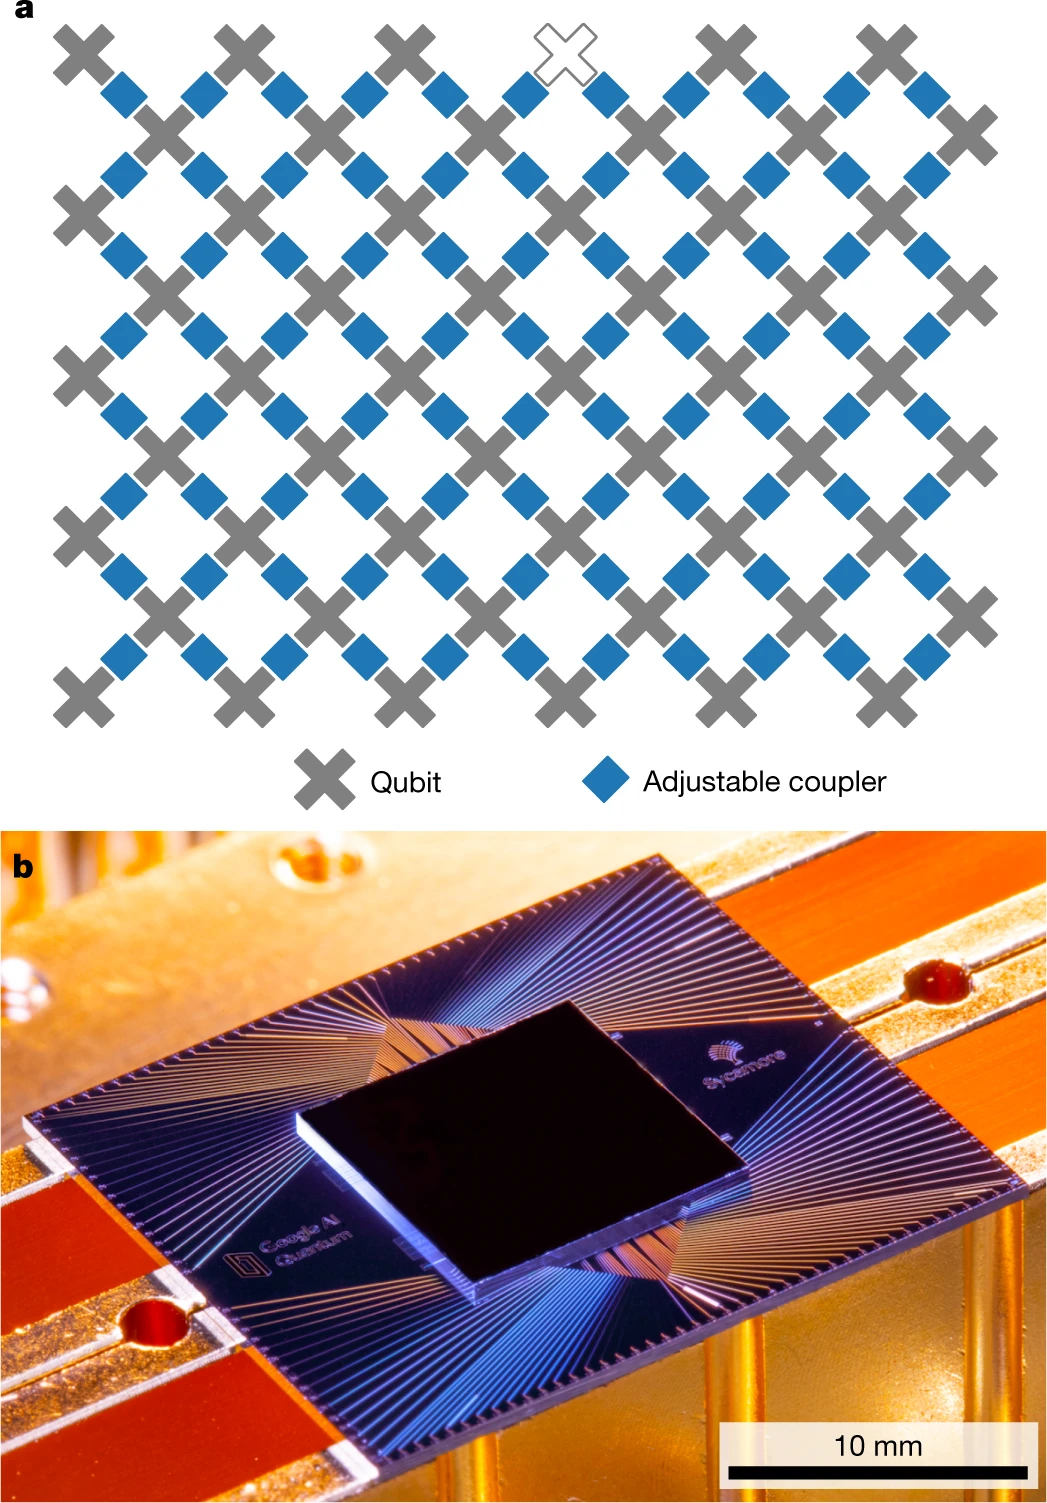
\includegraphics[width=0.7\linewidth]{img/SycamoreChip.png}
    \caption{Sycamore Chip von Google}
    \label{fig:Sycamore}
\end{figure}

\subsubsection{Superleitenden Qubits}
\label{subsub:superleiter}
Quantencomputer mit Supraleitern funktionieren mit elektrischen Schaltkreisen, die bei temperaturen nahe dem absoluten Nullpunkt betrieben werden. Solche temperaturen sind nötig
um die supraleitende Eigenschaft aufrecht zu erhalten.\\

Zwei häufig benutze Qubit-Typen dieser elektrischen Schaltkreisen sind:\\
\textbf{Transmon-Qubits}, basiert auf der Ladung des Energieniveaus welche durch eine Josephson-Junktion kontrolliert wird.\\
\textbf{Flux-Qubits} werden auch durch Josephson-Junktions kontrolliert, beruhen jedoch auf dem magnetischen Fluss in der Schleife.\\

Beide Ansätze basieren auf dem \textbf{Josephson-Effekt}, welcher auftritt wenn ein supraleitender Strom durch eine dünne Isolierschicht zwischen zwei Supraleitern fließt.\\
Dieser Effekt hat zur folge das eine nichtlineare Spannung-Stom-Beziehung erntsteht und für die Manipulation von Qubits genutzt wird.\\

\begin{figure}[H]
    \centering
    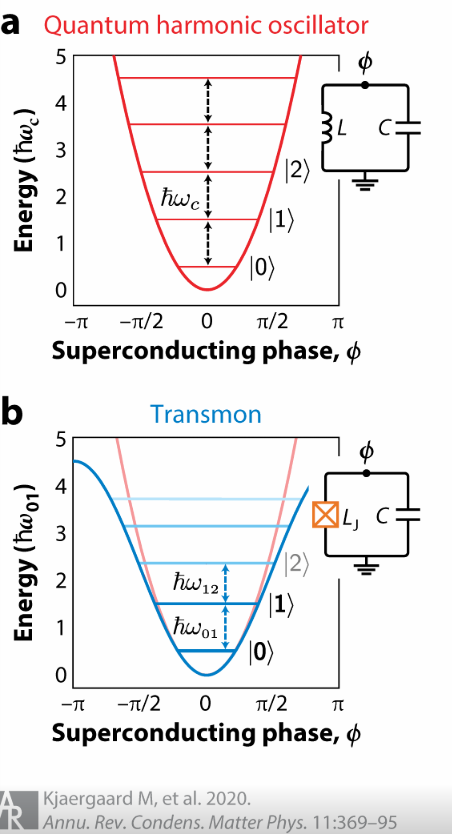
\includegraphics[width=0.75\linewidth]{img/JJ.png}
    \caption{Josephson-Effekt mit einem Josephson Junktion}
    \label{fig:Josephson-junktion}
\end{figure}

In der vorliegenden Abbildung wird der unterschied zwischen einer harmonischen Quantenschwankung (a) und der nicht Lineare Schwankung des Energieniveau der Josephson Junktion (b) abgebildet.\\

Der Phasenunterschied bei der harmonischen oscellation, gekennzeichnet als $\hbar\omega_c$, ist identisch. Auf der Abbildung ist zu sehen das das Energieniveau der Phasen zwischen $\ket{0} \leftrightarrow \ket{1}$
und $\ket{1} \leftrightarrow \ket{2}$ identisch ist, und dadurch nicht unterschieden werden kann zwischen welche Phase gewechselt wurde.\\

Mit einer Josephson Junktion kann jedoch eine nichtlineare Schwankung des Energieniveaus erreicht werden, welche auf der Abbildung als orangenes  gekennzeichnet ist (b).
Durch diese nichtlineare Schwankung ist das Energieniveau zwischen den Phasen $\ket{0} \leftrightarrow \ket{1}$ und $\ket{1} \leftrightarrow \ket{2}$ unterschiedlich und kann somit unterschieden werden.
Der als $\hbar\omega_{01}$ gekennzeichnete Energieunterschied ist unser Qubit\\

\textbf{Steuerung und Auslesung}\\
Die Steuerung der Josephson-Junktion erfolgt durch Mikrowellenpulse, welche die Energie des Qubits verändern. Die Auslesung erfolgt durch eine Mikrowellenresonanz, welche die Energie des Qubits misst.\\

\subsubsection{Quantenpunkte}
\label{subsub:quantenpunkte}
Quantencomputer basierend auf Quantenpunkten auch Quantum-Dot genannt nutzen winzige Halbleiterstrukturen um Qubits zu realisieren.
Quantum-Dots sind künstlich erzeugte Nano-Partikel, in denen Elektronen in drei Dimensionen eingeschlossen sind, was zu quantisierten Einergiezuständen führt.\\

Die größe eines Quantum-Dots typischerweise 2-10 Nanometer, und es schließt eine kleine Anzahl oder ein einzelnes Elektron ein.
Für die fertigung werden oftmals Galliumarsenid (GaAs) oder Silizium (Si) verwendet. Der physikalische einschluss der Elektronen schränkt ihre
Bewegung stark ein, wodurch ein quantisiertes Energienivea entsteht. Dies ähnelt den Energieniveaus eines Atoms, weswegen Quantum-Dots auch als künstliche Atome bezeichnet werden.\\

Die Zustände der Qubits werden durch die Eigenschaften einzelner Elektronen in den Quantum Dots definiert. Es gibt zwei Hauptansätze zur Realisierung von Qubits mit Quantum Dots.\\

\textbf{Ladungs-Qubits}\\
Der Ladungszustand eine Quantum Dots kann als Qubit verwendet werden. Die Ladung eines Elektrons kann entweder 0 oder 1 sein, was als $\ket{0}$ und $\ket{1}$ interpretiert wird.
Für eine messung wird der Ladungszustand mit einer Kapazitätsmessung der Tunnelströme ermittelt.
Für die Manipulation des Qubits werden elektrische Felder verwendet, um die Elektronen in den Quantum Dots zu bewegen.\\

Diese Methode ist durch die Ladungsquantisierung sehr genau, jedoch auch sehr empfindlich gegenüber Störungen durch die Umgebung.\\

\textbf{Spin-Qubits}\\
Die Spin-Eigenschaften von Elektronen in Quantum Dots können auch als Qubit verwendet werden. Hierbei sind die beiden Spinrichtungen($\uparrow$ für Spin-Up und $\downarrow$ für Spin-Down)
diese beiden Spinrichtungen entsprechen den Zuständen $\ket{0}$ und $\ket{1}$. Und die kombination aus beiden Zuständen ergibt eine Superposition.\\

\begin{figure}[H]
    \centering
    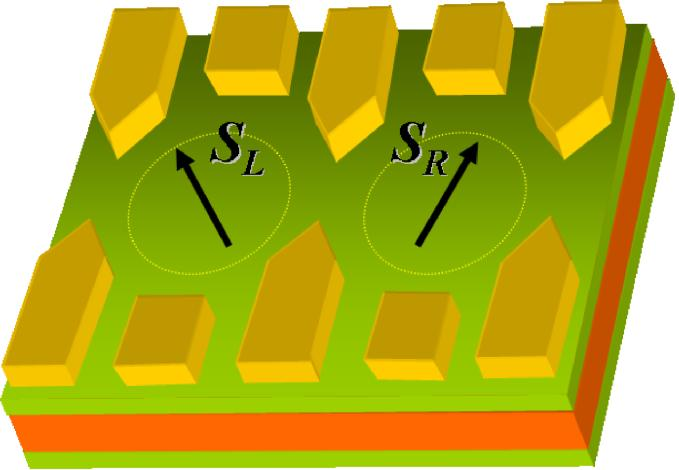
\includegraphics[width=0.75\linewidth]{img/QD.png}
    \caption{Ein doppel Quantum-Dot Qubit}
    \label{fig:double-Quantum-Dot}
\end{figure}

In der Abbildung ist ein doppel Quantum-Dot Qubit dargestellt. Sowohl in $S_L$ als auch $S_R$ befinden sich Elektornen. Beide können seperat von einander, sowohl im Spin als auch Ladung, manipuliert werden.
Durch die Physikalische nähe der beiden Quantum-Dots können durch Tunnelkopplung und Austauschwechselwirkung die beiden Qubits miteinander verschränkt werden.\\

Die umsetzung dieser Methode beschränkt such hauptsächlich auf die Spin variante. Der Grund dafür ist das Durch die hohe ladungsanforderung der Ladungsvariante die Qubits sehr empfindlich gegenüber Störungen sind.
Außerdem sind die Nachteile der Spin variante gegenüber der Ladungsvariante nicht so gravierend.\\
Jedoch sind die größten herausforderungen die Herstellung der Halbleiterstrukturen und die Kontrolle der Elektronen in den Quantum-Dots.
Damit ist der Größte vorteil, die hohe Skalierbarkeit, auch der größte nachteil, da die Herstellung und Kontrolle von vielen Quantum-Dots sehr aufwendig und schwierig ist.\\

\subsubsection{Topologische Quantencomputer}
\label{subsub:topologische_quantencomputer}
Der Ansatz von Topologischen Quantencomputern ist völlig anders als die bisher genannten. Im gegensatz zu diesen, welche auf eigenschaften einzelner Elektronen oder Energieniveaus basieren, basieren Topologische Quantencomputer auf topologischen Eigenschaften von Materie.\\
Diese Methode soll das Problem der Dekoheränz minimieren, indem sie Qubits aus Majorana-Partikeln aufbauen.\\

\textbf{Topologie in der Physik}\\
In einem Physikalischem System beschreibt die Topologie die Eigenschaften welche sich nicht durch deformiermation verändern lassen.
Ein Beispiel hierfür ist ein Kaffeebecher, welcher sich durch verformung in eine Donutform umwandeln lässt, beide haben die Topologische Eigenschaft eines Loches.
Daraus folgernd ist es nicht möglich ein Kaffeebecher oder ein Donut in eine Kugel zu verformen ohne die Topologische Eigenschaft zu verändern.\\

\textbf{Funktionsweise}\\
Die physikalische Grundlage für topologische Quantencomputer liegt in speziellen Materialien und Systemen, die topologische Materiephasen unterstützen.
Ein prominentes Beispiel ist die Verwendung von Majorana-Quasiteilchen, die in bestimmten Supraleitern auftreten können.\\

\begin{figure}[H]
    \centering
    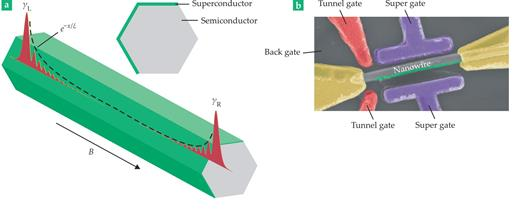
\includegraphics[width=0.75\linewidth]{img/Majorana.png}
    \caption{Nanowire mit Majorana-Quasiteilchen}
    \label{fig:Majorana}
\end{figure}

In der Abbildung ist ein Nanowire dargestellt, welcher durch ein Supraleiter und ein Magnetfeld in eine topologische Phase gebracht wird.
Diese Art von Partikel treten immer als Paar auf und bilden eine Art Brücke zwischen den Elektronen. Diese Brücke wird durch die topologischen Eigenschaften der Majorana-Partikel stabilisiert und ist somit weniger anfällig gegenüber Störungen.\\

\begin{tcolorbox}[title=Kommentar,
    title filled=false,
    colback=cyan!5!white,
    colframe=cyan!75!black]
    Die Vertiefung der durch den Quanten-Hall Effekt entsteht wird nur oberflächlich behandelt. Ist jedoch essentiell für die Funktionsweise von Topologischen Quantencomputern.
\end{tcolorbox}

\textbf{Verpflechtung}\\
Braiding ist der Prozess, bei dem die Majorana-Partikel miteinander verflochten werden, um die Quantenbits zu manipulieren. 
Dies Passiert auf einer zweidimensionalen Oberfläche, auf welcher die Majorana-Partikel miteinander verflochten werden.\\

\begin{figure}[H]
    \centering
    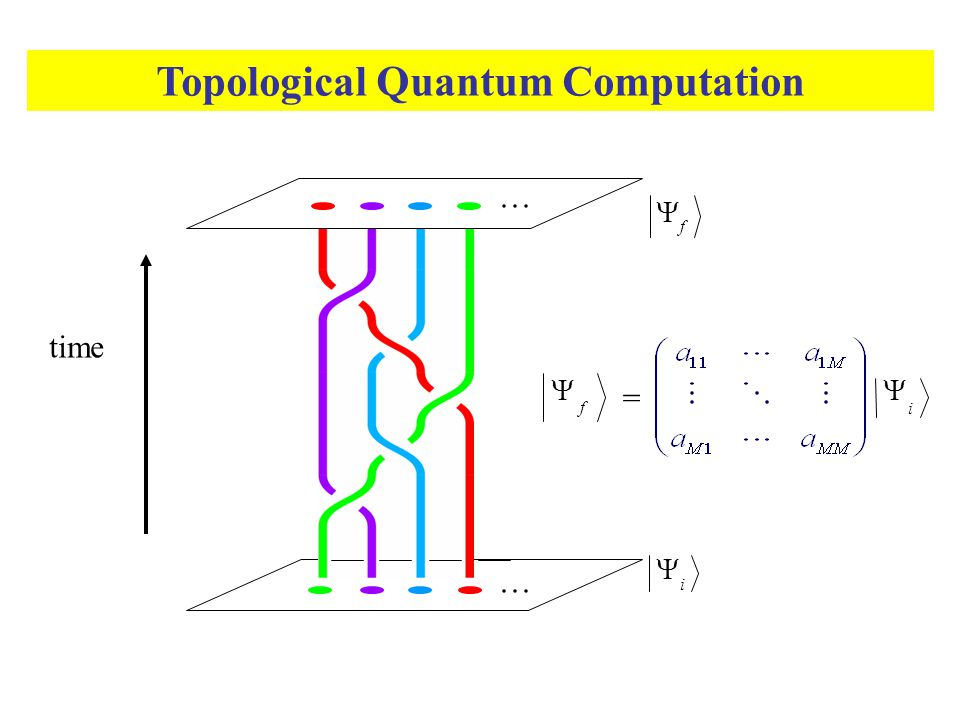
\includegraphics[width=0.75\linewidth]{img/TQC.png}
    \caption{Braiding von Majorana-Quasiteilchen}
    \label{fig:Braiding}
\end{figure}

Hierbei ist es wichtig in welcher reihenfolge da durch diese Reihenfolge Quantenoperationen realisiert werden.
Jede Verpflechtung entspricht einer Quantenoperation, und durch die Kombination von mehreren Verpflechtungen können beliebige Quantenoperationen realisiert werden.\\

Da die Informationen und Quantenoperationen in der Topologie steckt, sind sie gegenüber kleinen Fehlern in der Bewegung/Störungen unempfindlich.\\

\begin{tcolorbox}[title=Kommentar,
    title filled=false,
    colback=cyan!5!white,
    colframe=cyan!75!black]
    Die Technische umsetzung von Topologischen Quantencomputern ist deutlich komplizierter als in diesem Abschnitt oberflächlich beschrieben ist.\\
    Bisher hat nur Google einen Topologischen Quantencomputer vorgestellt, welcher jedoch noch nicht in der Lage ist Quantenoperationen durchzuführen.
\end{tcolorbox}

\subsection{Quantum Error Correction}
\label{sub:quantum_error_correction}
Quantum Error Correction oder auf QEC genannt ist grundlegend wichtig für die funktionellen betrieb eines Quantencomputers. Wie bereits in den vorherigen Abschnitten beschrieben,
sind Qubits sehr anfällig gegenüber Dekoheränz und Quantenrauschen.\\

\textbf{Warum ist Fehlerkorrektur notwendig}\\
Fehler treten in Quantencomputer durch drei Hauptquellen auf.\\
1. \textbf{Dekoheränz} welche durch äußere Einflüsse wie Temperaturschwankungen oder elektromagnetische Felder die koheränten Eigenschaften der Qubits zerstört.\\
2. \textbf{Phasen-Flip-Fehler} Hierbei werden die Phasenwinkel zwischen den Quantenzuständen verändert($\ket{0}\rightarrow\ket{0},\ket{1}\rightarrow-\ket{1}$).\\ 
3. \textbf{Bit-Flip-Fehler} Hierbei werden die Zustände der Qubits verändert ($\ket{0}\rightarrow\ket{1},\ket{1}\rightarrow\ket{0}$).\\

Bei der Fehlerkorrektur von Quantencomputern ist jedoch zu beachten das dies nicht wie bei herkömmlichen Computern da durch das No-Cloning-Theorem keine Quanteninformationen kopier werden können.\\

\textbf{Grundprinzip}\\
Quanten-Fehlerkorrektur verwendet \textbf{Redundanz}, um Fehler zu detektieren und zu korrigieren, ohne das die eigentliche Quanteninformationen direkt ausgelesen werden.\\

Eine art der Redundanz ist der Steane-Code, welcher auf 7 Qubits basiert. Dieser zusammenschluss aus 7 Physischen Qubits bildet ein logisches Qubit,
welche ein fehler auf einem der 7 Qubits korrigieren kann. Treten jedcoh mehrere Fehler auf, kann der Steane-Code diese nicht korrigieren.\\

\begin{figure}[H]
    \centering
    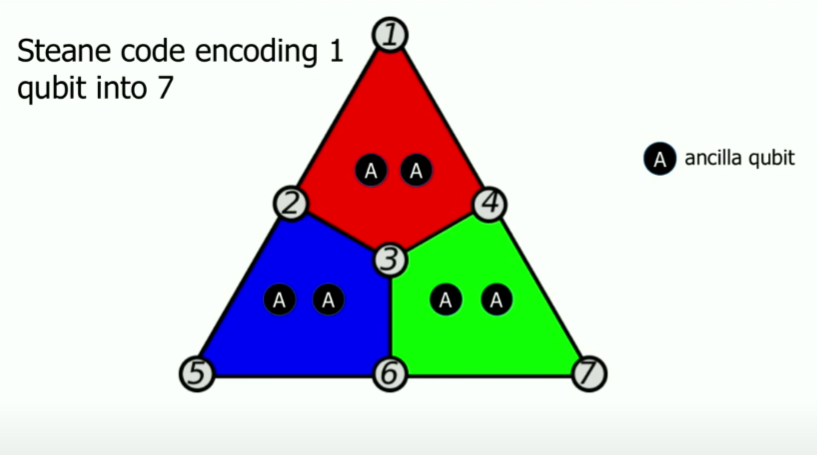
\includegraphics[width=0.75\linewidth]{img/Steane.png}
    \caption{Steane-Code}
    \label{fig:Steane}
\end{figure}

Um die Qubits zu überwachen werden zusätzliche Qubits benötigt, da das direkte auslesen dieser den Quantenzustand zerstören würde.
Diese zusätzlichen Qubits werden als \textbf{Ancilla qubit} bezeichnet und mit den eigentlichen Qubits verschränkt.\\

\textbf{Fehlertoleranz}\\
Diese Herangehensweise ist jedoch auch nicht perfekt, die Ancilla Qubits sind gleichermaßen anfällig gegenüber Fehlern wie die eigentlichen Qubits.\\

\begin{figure}[H]
    \centering
    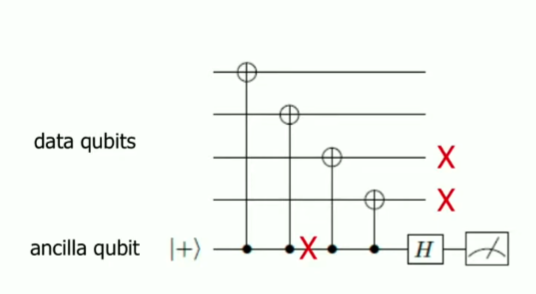
\includegraphics[width=0.75\linewidth]{img/Fehlertoleranz.png}
    \caption{Fehlertoleranz von Ancilla Qubits}
    \label{fig:Fehlertoleranz}
\end{figure}

Dieses Abbildung zeigt wie eine einzelner Fehler in einem CNOT Gatter auf dem Ancilla bit Messung der daten qubits als Fehler kennzeichnet obwohl diese nicht fehlerhaft sind.\\
Die Folge hieraus ist das die Fehlerkorrektur mit wenigen Qubits nicht ausreicht, um diesen Logischen Qubit volkommen Fehlerfrei zu halten.\\

Hierbei werden zwischen zwei Parität checks unterschieden. Ein $Z$ und $X$ Parität welcher festlegt ob der Fehler in den Ancilla Qubits CNOT Gattern oder den Daten Qubits aufgetreten ist.\\

\textbf{Suface Code}\\
Eine weitere Methode zur Fehlerkorrektur ist der Surface Code, welcher auf einem 2D Gitter von Qubits basiert.
Dieser Code ist in der Lage Fehler zu detektieren und zu korrigieren, solange die Fehlerdichte unter einem bestimmten Wert bleibt.\\

Die Größe des Surface Codes ist variabel und kann Skaliert werden, um die Fehlerkorrektur zu verbessern.
Es gibt jedoch ein Threshold an der die vergößerung des Codes keine Verbesserung mehr bringt.
Durch die vorher besprochene Fehlertoleranz der Ancilla Qubits wird die Effektivität des Surface Codes gedeckelt, die Fehler in der Korrektur an sich werden hierbei mehr als wenn keine Korrektur vorgenommen wird, und es würde keinen sinn ergeben den Surface Code weiter zu vergößern.\\

Die Nachfolgende Abbildung eines Surface Codes des grades $d=3$ zeigt wie die Qubits in einem 2D Gitter angeordnet sind und wie die Fehlerkorrektur durchgeführt wird.
Jede überschneidung des Gatters stellt ein Physichen Qubit dar. Die Kreise in den Quadraten sind die Ancilla Qubits, welche die Fehlerkorrektur durchführen.\\

\begin{figure}[H]
    \centering
    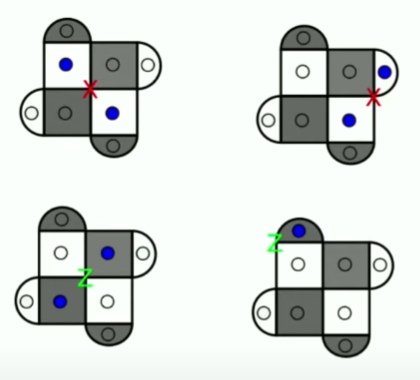
\includegraphics[width=0.6\linewidth]{img/Errors.png}
    \caption{Fehlerkorrektur durch Surface Code des Grades $d=3$}
    \label{fig:Surface-Code}
\end{figure}

Ancilla Qubits in einem Weißen feld prüfen die Qubits auf ein logischen $X$ und Ancilla Qubits in einem Schwarzen Feld prüfen die Qubits auf ein logisches $Z$.\\

Ancilla Qubits die ein Fehler erkennen werden als Blau markiert, und durch die Position dieser und für welche daten Qubits diese zuständig sind wissen wir welche Qubits fehlerhaft sind.\\

\textbf{Praktische Umsetzung}\\
Am 09.12.2024 hat Google den ersten selbst Korrigierenden Quantencomputer vorgestellt, welcher auf dem Surface Code basiert.
Der Chip namens \textbf{Willow} basiert auf 105 Physischen Qubits wobei diese auf der 7x7 Surface Code Architektur aufbaut.
Dies Resultiert in 49 Qubits welche deutlich weniger anfälliggegen fehler sind als Phyische Qubits, die restlichen Qubits werden für Parität und error Korrektur gebraucht.\\

\begin{figure}[H]
    \centering
    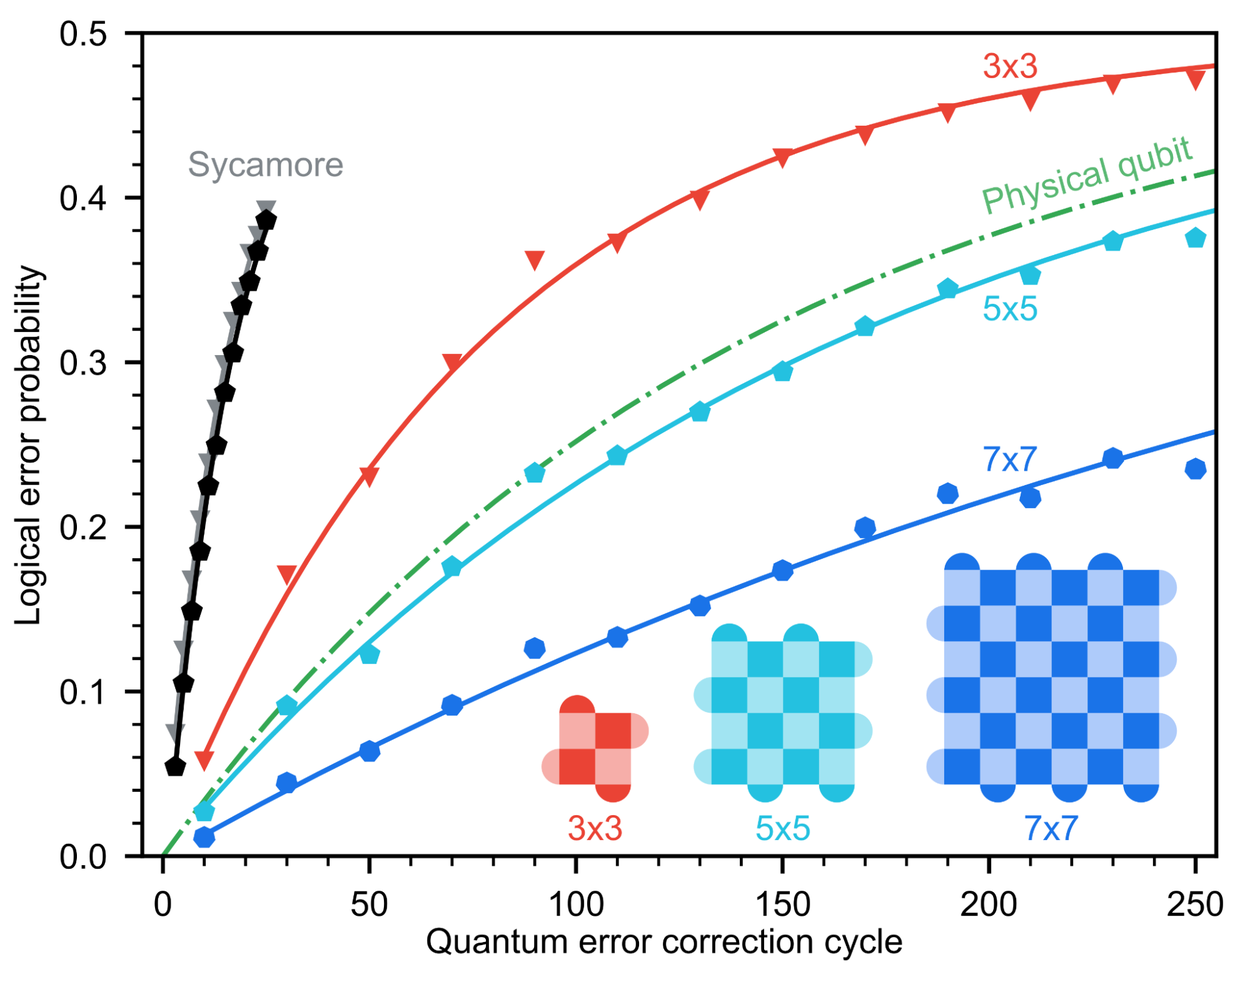
\includegraphics[width=0.7\linewidth]{img/Surface-Code-Scaling.png}
    \caption{Error Korrektur des 7x7 Surface Code}
    \label{fig:Willow}
\end{figure}

Außerdem wurde durch die anwendung des Surface Codes die $T_1$ zeit von $20\mu s$ auf $68\mu s\pm13\mu s$ erhöht und ermöglich hierdurch mehr Operationen pro Qubit.\\